\chapter{\label{app:7-chargetransition}Charge transition diagram for metastable iodine interstitial defects}

\begin{figure}[h!]   %includes H-centre schematic
\centering
  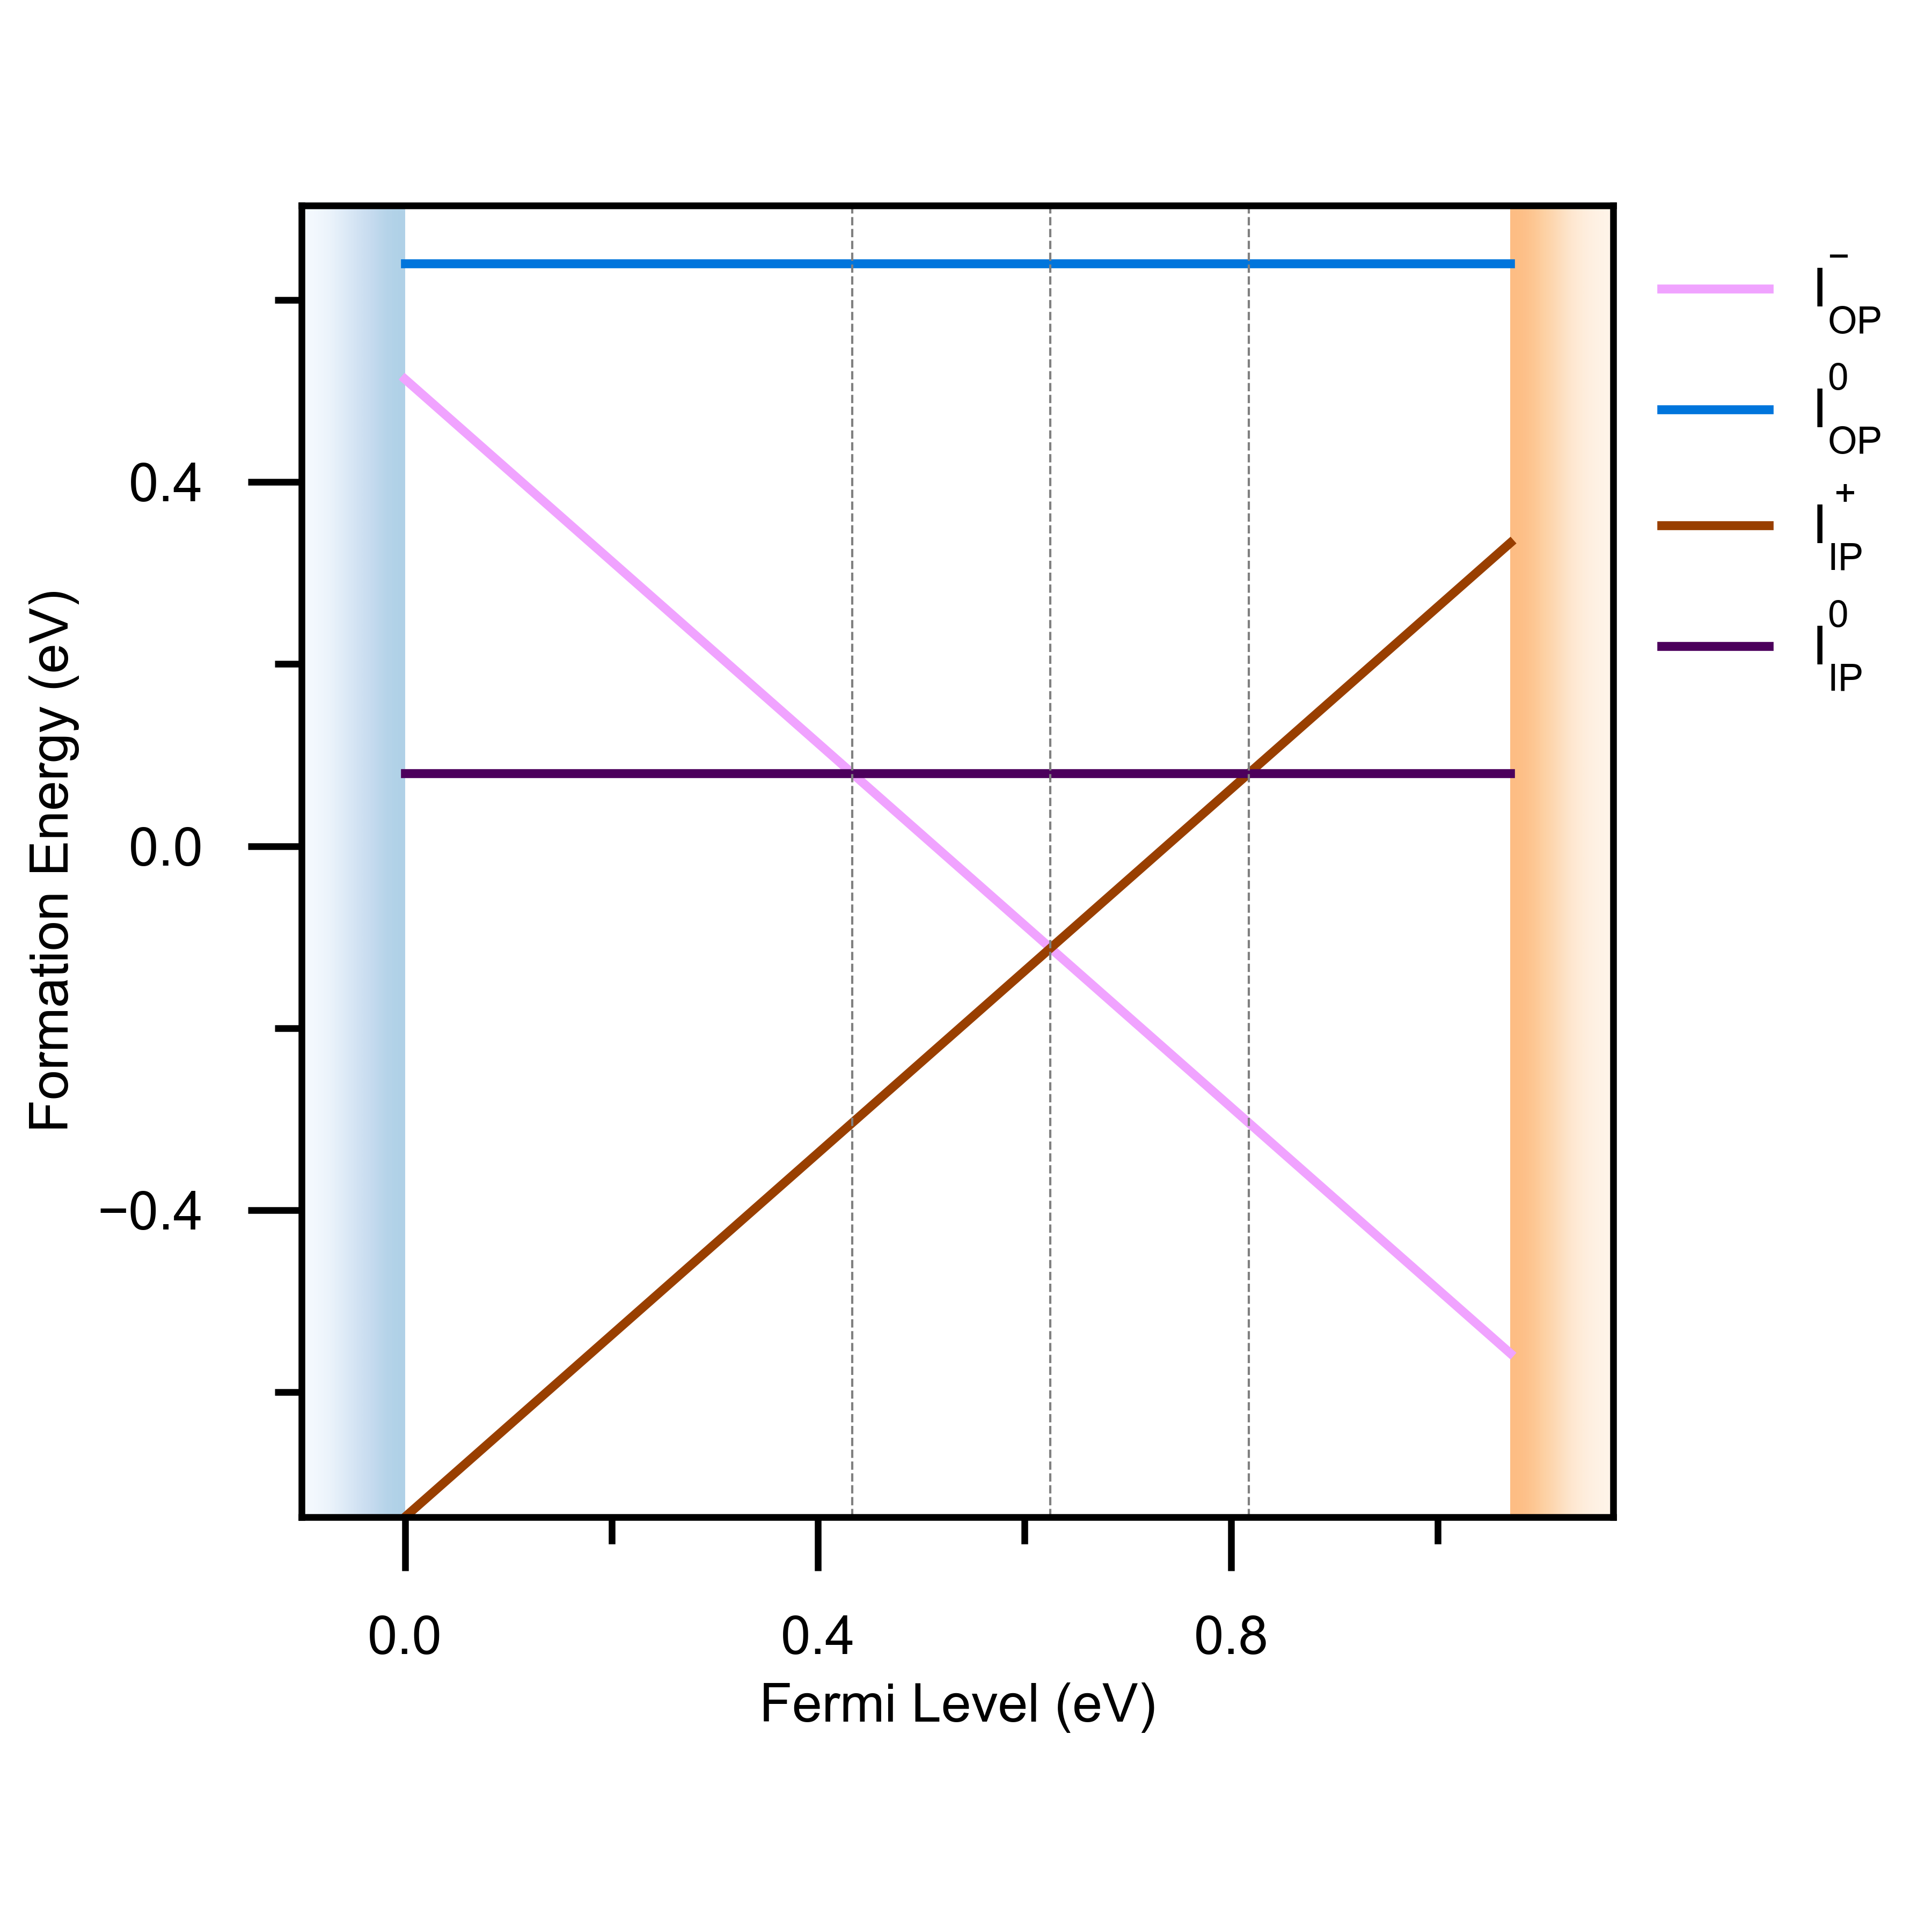
\includegraphics[width=0.7\columnwidth]{figures/ap7/charge_transition_HSE_meta.png}
  \caption[Charge transition diagram for metastable iodine interstitial defects in MAPI]{Charge transition diagram for the metastable iodine interstitial defects in MAPI. The defect geometries correspond to those in the solid boxes in Figure \ref{relaxation_workflow} ($\mathrm{I}_\mathrm{i}^{+,\mathrm{IP}}$,$\mathrm{I}_\mathrm{i}^{-\mathrm{OP}}$,$\mathrm{I}_\mathrm{i}^\mathrm{IP}, \mathrm{I}_\mathrm{i}^\mathrm{OP}$). Lower energy defects were found and the charge transition diagrame for these are reported in the main text. For the metastable defects reported here three charge transitions are in the bandgap, in line with the previous literature.\autocite{Du2015,Meggiolaro2018}}
\label{charge_transition_meta}
\end{figure}